\documentclass[a4paper,12pt]{article}
\usepackage[utf8]{inputenc} 
\usepackage{amsmath}
\usepackage[a4paper, margin=0.6in,top=0.3in, bottom=0.3in]{geometry} % Adjust the margin here
\usepackage{multirow}
\usepackage{circuitikz}
\usepackage{nopageno}
\usepackage{graphicx} % Add this line to include graphics
\usepackage{tikz} % Add this line to use TikZ for drawing
\usepackage{tikz-3dplot} % Add this line to use 3D plotting
\setlength{\parindent}{0pt} % Set global no indent
    
\title{{\large Department of Physics, FNSPE, CTU in Prague} \\
                  02YELMA - Electricity and Magnetism \\ 
          {\Large \textbf{Final Exam}}\vspace{-1cm}}
\date{15.6.2026 / 14:00 - 16:30}
\author{}

\begin{document}

\maketitle
\vspace{-0.8cm}

\noindent
\begin{minipage}[t]{0.58\textwidth}
\vspace{0pt}
\textbf{Q1:} Resistors, inductors, and capacitors are connected with an alternating voltage source $V(t)~=~V_0 \sin(\omega t)$ as shown in the figure. Assume that the circuit is ideal and there is no mutual inductance between the inductors.
\begin{enumerate}
    \item[(a)] Write down the differential equation governing \underline{the current} $I(t)$ in the circuit.
    \item[(b)] To obtain the greatest possible current amplitude, what should be the value of $\omega$? 
    \item[(c)] Given that the steady-state current is $I(t)=I_0 \sin(\omega t + \phi)$, find the average energy dissipation in the circuit at the resonance frequency per unit time? 
\end{enumerate}
\end{minipage}\hfill
\begin{minipage}[t]{0.4\textwidth}
\vspace{0pt}
\centering
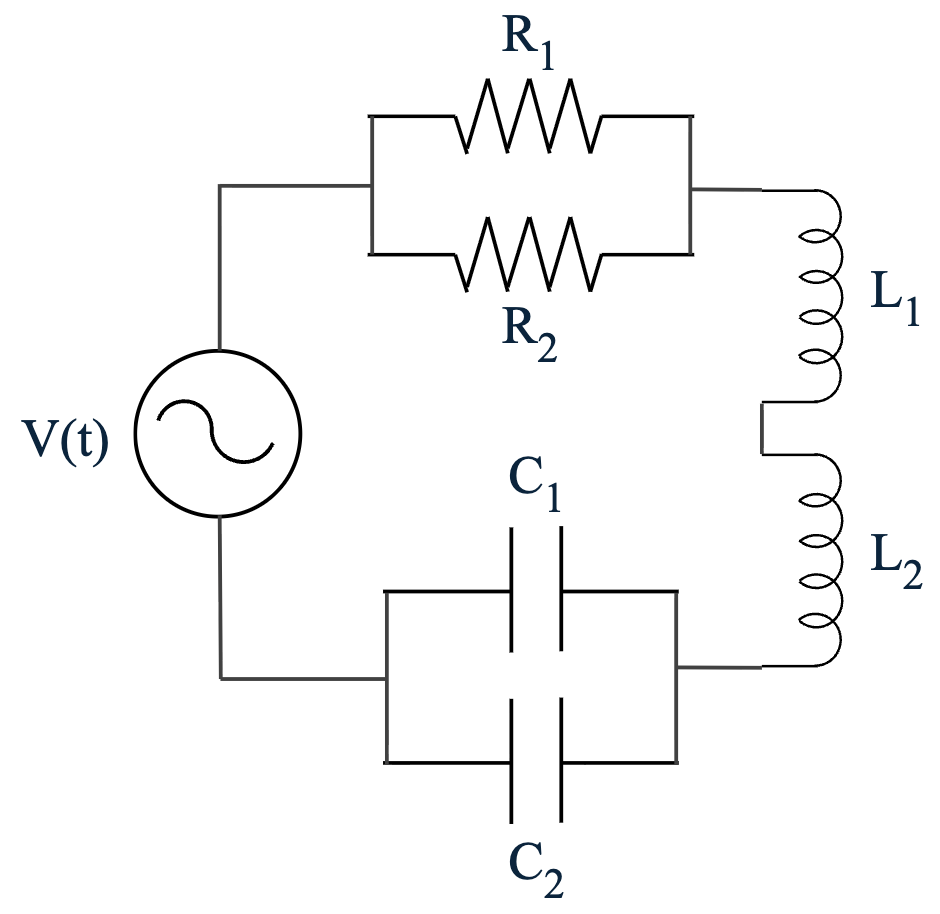
\includegraphics[width=\linewidth]{rlc.png}
\end{minipage}

\vspace*{0.3cm}
\textbf{Q2:} A long coaxial capacitor consists of two concentric cylindrical conductors with radii $a$ and $b$ ($a < b$) and vacuum spacing. It is driven by a time-dependent voltage $V(t) = V_0 \cos(\omega t)$ applied between the inner and outer conductors. Assume cylindrical symmetry and neglect edge effects. Determine the electric field $\vec{E}(r,t)$ in the regions $a < r < b$ and $r > b$.

\vspace*{0.3cm}
\textbf{Q3:} A parallel-plate capacitor is at rest in frame $S'$, producing a uniform electric field $\vec{E}' = E_0 \hat{y}'$. Frame $S'$ moves with constant velocity $\vec{v} = v \hat{x}$ relative to laboratory frame $S$. Determine the electric field $\vec{E}$ and magnetic field $\vec{B}$ in frame $S$ interpret the result in terms of the motion of the charges in the capacitor.
\emph{Given:} $E_{\parallel} = E'_{\parallel}$, $E_{\perp} = \gamma (E'_{\perp} - \vec{v} \times \vec{B}')$, $B_{\parallel} = B'_{\parallel}$, and $B_{\perp} = \gamma (B'_{\perp} + \frac{1}{c^2} \vec{v} \times \vec{E}')$, where $\gamma = 1/\sqrt{1 - v^2/c^2}$ is the Lorentz factor and directions $\parallel$ and $\perp$ are defined with respect to the velocity $\vec{v}$.

\noindent

\vspace*{0.3cm}

\noindent
\begin{minipage}[t]{0.48\textwidth}
\vspace{0pt}
\textbf{Q4:} A conducting rod of length \(L\) and resistance \(R\) slides without friction on two parallel conducting rails that are connected by a resistor \(R_0\), forming a closed rectangular circuit. The entire setup lies in the \(xy\)-plane. A uniform magnetic field $\vec{B}=B_0 \hat{z}$ is directed perpendicular to the plane of the circuit. Initially, the rod moves to the right with velocity $v(t)=v_0 e^{-\alpha t}$ where \(v_0\) and \(\alpha\) are positive constants. Neglect the resistance of the rails.


\end{minipage}\hfill
\begin{minipage}[t]{0.5\textwidth}
\vspace{0pt}
\centering
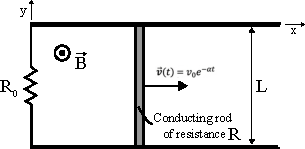
\includegraphics[width=\linewidth]{rail.pdf}
\end{minipage}
\begin{enumerate}
    \item[(a)] Determine the motional electromotive force (EMF) induced in the circuit and the induced current $I(t)$ (including its direction) as a function of time.
    
    \item[(b)] Calculate the magnetic force acting on the rod as a function of time. Verify that its direction is consistent with Lenz's law.
    
    \item[(c)] Suppose the prescribed velocity is maintained  by an external agent acting on the rod (of mass $m$), determine the electrical power $P_{\text{elec}}$ dissipated in the circuit  and the mechanical power $P_{\text{ext}}$ supplied by the agent verify the energy conservation and comment on the sign of $P_{\text{ext}}$.
\end{enumerate}

\end{document}

